\chapter{Numbers 19}

\begin{figure}
  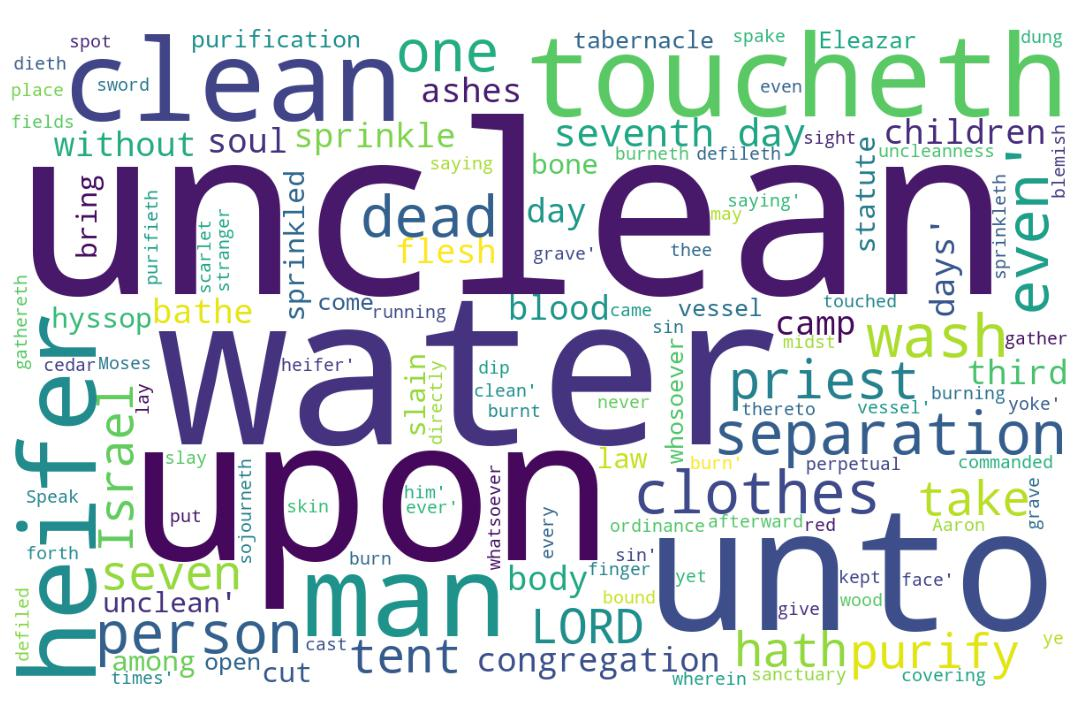
\includegraphics[width=\linewidth]{04OT-Numbers/Numbers19-WordCloud.jpg}
  \caption{Numbers 19 Word Cloud}
  \label{fig:Numbers 19 word Cloud}
\end{figure}



\marginpar{\scriptsize \centering \fcolorbox{bone}{lime}{\textbf{A RED HIEFER}}\\ (Numbers 19)
\begin{compactenum}[I.][8]
    \item  \textbf{Days} \index[scripture]{Numbers!Num 19:11} \index[scripture]{Numbers!Num 19:12} \index[scripture]{Numbers!Num 19:14}\index[scripture]{Numbers!Num 19:16}\index[scripture]{Numbers!Num 19:19} (Numbers 19:11, 12, 14, 16, 19) -- the typology of the third day and the seventh day
    \item  \textbf{Defilement} \index[scripture]{Numbers!Num 19:13} \index[scripture]{Numbers!Num 19:20} (Numbers 19:13, 20) 
    \item  \textbf{Destinations} \index[scripture]{Numbers!Num 19:03} \index[scripture]{Numbers!Num 19:07}\index[scripture]{Numbers!Num 19:09} (Numbers 19:3, 7, 9) -- inside the camp, outside the camp
    \item  \textbf{Designees}  -- the priest, the clean person, the unclean person, the dead body
    \item  \textbf{Ordinance}  \index[scripture]{Numbers!Num 19:02} (Numbers 19:2) 
    \item  \textbf{Defect} Free \index[scripture]{Numbers!Num 19:02} (Numbers 19:2) 
\end{compactenum}}

%[cmyk]{0.99998,1,0,0}{

\footnote{\textcolor[rgb]{0.00,0.25,0.00}{\hyperlink{NumbersTOC}{Return to end of Table of Contents.}}}\footnote{\href{https://audiobible.com/bible/numbers_19.html}{\textcolor[cmyk]{0.99998,1,0,0}{Numbers 19 Audio}}}\textcolor[cmyk]{0.99998,1,0,0}{And the LORD spake unto Moses and unto Aaron, saying,}
[2] \textcolor[cmyk]{0.99998,1,0,0}{This \emph{is} the ordinance of the law which the LORD hath commanded, saying, Speak unto the children of Israel, that they bring thee a red heifer without spot, wherein \emph{is} no blemish, \emph{and} upon which never came yoke:}
[3] \textcolor[cmyk]{0.99998,1,0,0}{And ye shall give her unto Eleazar the priest, that he may bring her forth without the camp, and \emph{one} shall slay her before his face:}
[4] \textcolor[cmyk]{0.99998,1,0,0}{And Eleazar the priest shall take of her blood with his finger, and sprinkle of her blood directly before the tabernacle of the congregation seven times:}
[5] \textcolor[cmyk]{0.99998,1,0,0}{And \emph{one} shall burn the heifer in his sight; her skin, and her flesh, and her blood, with her dung, shall he burn:}
[6] \textcolor[cmyk]{0.99998,1,0,0}{And the priest shall take cedar wood, and hyssop, and scarlet, and cast \emph{it} into the midst of the burning of the heifer.}
[7] \textcolor[cmyk]{0.99998,1,0,0}{Then the priest shall wash his clothes, and he shall bathe his flesh in water, and afterward he shall come into the camp, and the priest shall be unclean until the even.}
[8] \textcolor[cmyk]{0.99998,1,0,0}{And he that burneth her shall wash his clothes in water, and bathe his flesh in water, and shall be unclean until the even.}
[9] \textcolor[cmyk]{0.99998,1,0,0}{And a man \emph{that} \emph{is} clean shall gather up the ashes of the heifer, and lay \emph{them} up without the camp in a clean place, and it shall be kept for the congregation of the children of Israel for a water of separation: it \emph{is} a purification for sin.}
[10] \textcolor[cmyk]{0.99998,1,0,0}{And he that gathereth the ashes of the heifer shall wash his clothes, and be unclean until the even: and it shall be unto the children of Israel, and unto the stranger that sojourneth among them, for a statute for ever.}\\
\\
\P \textcolor[cmyk]{0.99998,1,0,0}{He that toucheth the dead body of any man shall be unclean seven days.}
[12] \textcolor[cmyk]{0.99998,1,0,0}{He shall purify himself with it on the third day, and on the seventh day he shall be clean: but if he purify not himself the third day, then the seventh day he shall not be clean.}
[13] \textcolor[cmyk]{0.99998,1,0,0}{Whosoever toucheth the dead body of any man that is dead, and purifieth not himself, defileth the tabernacle of the LORD; and that soul shall be cut off from Israel: because the water of separation was not sprinkled upon him, he shall be unclean; his uncleanness \emph{is} yet upon him.}
[14] \textcolor[cmyk]{0.99998,1,0,0}{This \emph{is} the law, when a man dieth in a tent: all that come into the tent, and all that \emph{is} in the tent, shall be unclean seven days.}
[15] \textcolor[cmyk]{0.99998,1,0,0}{And every open vessel, which hath no covering bound upon it, \emph{is} unclean.}
[16] \textcolor[cmyk]{0.99998,1,0,0}{And whosoever toucheth one that is slain with a sword in the open fields, or a dead body, or a bone of a man, or a grave, shall be unclean seven days.}
[17] \textcolor[cmyk]{0.99998,1,0,0}{And for an unclean \emph{person} they shall take of the ashes of the burnt heifer of purification for sin, and running water shall be put thereto in a vessel:}
[18] \textcolor[cmyk]{0.99998,1,0,0}{And a clean person shall take hyssop, and dip \emph{it} in the water, and sprinkle \emph{it} upon the tent, and upon all the vessels, and upon the persons that were there, and upon him that touched a bone, or one slain, or one dead, or a grave:}
[19] \textcolor[cmyk]{0.99998,1,0,0}{And the clean \emph{person} shall sprinkle upon the unclean on the third day, and on the seventh day: and on the seventh day he shall purify himself, and wash his clothes, and bathe himself in water, and shall be clean at even.}
[20] \textcolor[cmyk]{0.99998,1,0,0}{But the man that shall be unclean, and shall not purify himself, that soul shall be cut off from among the congregation, because he hath defiled the sanctuary of the LORD: the water of separation hath not been sprinkled upon him; he \emph{is} unclean.}
[21] \textcolor[cmyk]{0.99998,1,0,0}{And it shall be a perpetual statute unto them, that he that sprinkleth the water of separation shall wash his clothes; and he that toucheth the water of separation shall be unclean until even.}
[22] \textcolor[cmyk]{0.99998,1,0,0}{And whatsoever the unclean \emph{person} toucheth shall be unclean; and the soul that toucheth \emph{it} shall be unclean until even.}
